\documentclass[tikz,border=8pt]{standalone}
\usepackage{pgfplots}
\pgfplotsset{compat=1.18}
\begin{document}
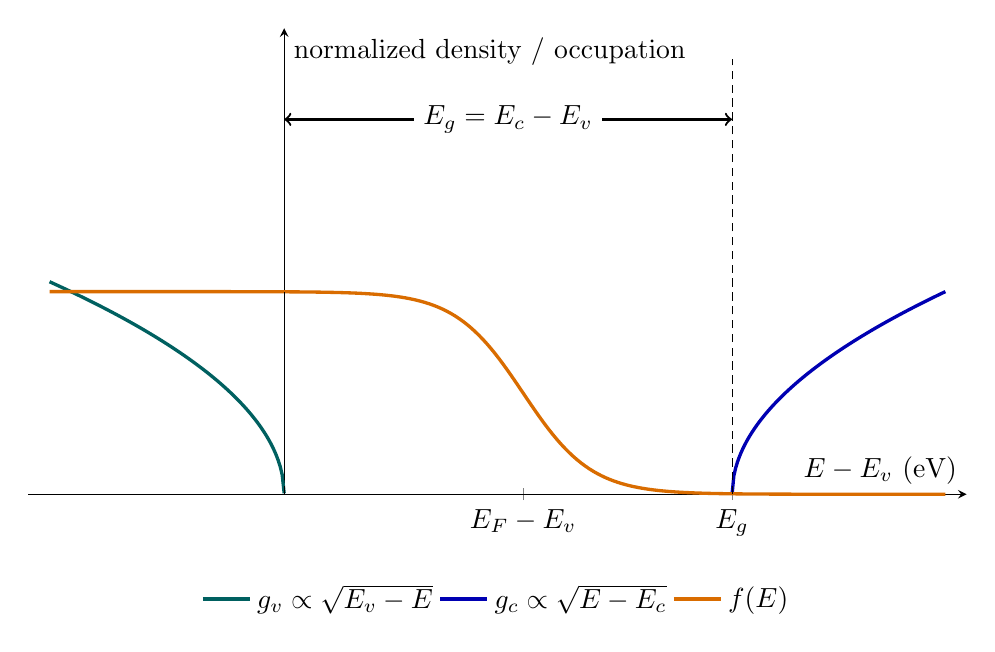
\begin{tikzpicture}
\begin{axis}[width=13.5cm,height=7.5cm,xmin=-1.2,xmax=3.2,ymin=0,ymax=2.3,
 axis lines=middle,xlabel={$E-E_v$ (eV)},ylabel={normalized density / occupation},
 xtick={0,1.12,2.1},xticklabels={$0$,$E_F-E_v$,$E_g$},ytick=\empty,
 legend style={at={(0.5,-0.17)},anchor=north,legend columns=3,draw=none},clip=false]
\addplot[very thick,teal!75!black,domain=-1.1:0,samples=120]{sqrt(-x)};
\addplot[very thick,blue!70!black,domain=2.1:3.1,samples=120]{sqrt(x-2.1)};
\addplot[very thick,orange!85!black,domain=-1.1:3.1,samples=220]{1/(1+exp((x-1.12)/0.16))};
\draw[densely dashed] (axis cs:0,0)--(axis cs:0,2.15);
\draw[densely dashed] (axis cs:2.1,0)--(axis cs:2.1,2.15);
\draw[<->,thick] (axis cs:0,1.85)--node[fill=white]{$E_g=E_c-E_v$}(axis cs:2.1,1.85);
\legend{$g_v\propto\sqrt{E_v-E}$,$g_c\propto\sqrt{E-E_c}$,$f(E)$}
\end{axis}
\end{tikzpicture}
\end{document}
